\documentclass[hyperref]{article}
%MS%%%%%%%%%%%%%%%%%%%% Article Format %%%%%%%%%%%%%%%%%
%+++++++++++++++++++++ Usepackage +++++++++++++++%%
\usepackage{graphicx} %% Package for Figure
\usepackage{float} %% Package for Float
\usepackage{amssymb}
\usepackage{amsmath}
\usepackage{mathtools}
\usepackage[thmmarks,amsmath]{ntheorem} %% If amsmath is applied, then amsma is necessary
\usepackage{bm} %% Bold Mathematical Symbols
\usepackage[colorlinks,linkcolor=cyan,citecolor=cyan]{hyperref}
\usepackage{extarrows}
\usepackage[hang,flushmargin]{footmisc} %% Let the footnote not indentation
\usepackage[square,comma,sort&compress,numbers]{natbib} %% Sort of References
\usepackage{mathrsfs} %% Swash letter
\usepackage[font=footnotesize,skip=0pt,textfont=rm,labelfont=rm]{caption,subcaption} 
%% Format of Caption for Tab. and Fig.
\usepackage{booktabs} %% tables with three lines
\usepackage{tocloft}
\usepackage{graphicx}
%+++++++++++++++ Proof etc. +++++++++++++++++++++++++%%
{%% Environment of Proof
	\theoremstyle{nonumberplain}
	\theoremheaderfont{\bfseries}
	\theorembodyfont{\normalfont}
	\theoremsymbol{\mbox{$\Box$}}
	\newtheorem{proof}{Proof}
}

\usepackage{theorem}
\newtheorem{theorem}{Theorem}[section]
\newtheorem{lemma}{Lemma}[section]
\newtheorem{definition}{Definition}[section]
\newtheorem{assumption}{Assumption}[section]
\newtheorem{example}{Example}[section]
\newtheorem{corollary}{Corollary}[section]
{%% Environment of Remark
	\theoremheaderfont{\bfseries}
	\theorembodyfont{\normalfont}
	\newtheorem{remark}{Remark}[section]
}
\usepackage{abstract}
\renewcommand{\abstractnamefont}{\Large\bfseries}
%\numberwithin{equation}{section} %% Number of Equation
%++++++++++++++++++++++++++++++++ Page format ++++++++++++++++++++++++++%%
\graphicspath{{figure/}}                                 %% Path of Figures
\usepackage[a4paper]{geometry}                           %% Paper size
\geometry{left=2.5cm,right=2.5cm,top=2.5cm,bottom=2.5cm} %% Margin
\linespread{1.2}                                         %% Line Spread
%MS%%%%%%%%%%%%%%%%%%%%%%%%%%%% End Format %%%%%%%%%%%%%%%%%%%%%%%%%%%%%%%%%%

%MS%%%%%%%%%%%%%%%%%%%%%%%%%%%%%%%%%%%%%%%%%%%
%MS                                         %%
%MS        The Main Body begins here        %%
%MS                                         %%
%MS%%%%%%%%%%%%%%%%%%%%%%%%%%%%%%%%%%%%%%%%%%%

%MS++++++++++++++++++++++++++++++ Title +++++++++++++++++++
\title{Assignment for EE5101/ME5401 Linear Systems}
\author{\textup{Yihui Chen}}
\begin{document}
	\begin{titlepage}
		\center
		\newcommand{\HRule}{\rule{\linewidth}{0.5mm}}
		
\includegraphics[width=8cm]{logo.png}\\[1cm] 
		\quad\\[1.5cm]
		\textsl{\Large National University of Singapore}\\[0.5cm] 
		\textsl{\large College of Design and Engineering}\\[0.5cm]
		\makeatletter
		\HRule \\[0.4cm]
		{ \huge \bfseries \@title}\\[0.4cm] 
		\HRule \\[1.5cm]
		\begin{minipage}{0.4\textwidth}
			\begin{flushleft} \large
				\emph{Author:}\\
				\@author 
			\end{flushleft}
		\end{minipage}
		~
		\begin{minipage}{0.4\textwidth}
			\begin{flushright} \large
				\emph{Supervisor:} \\
				\textup{Prof Yang}
			\end{flushright}
		\end{minipage}\\[3cm]
		\makeatother
		{\Large Assignment for EE5101/ME5401 Linear System}\\[0.5cm]
		{\large \emph{Matriculation Number: A0263115N}}\\[0.5cm]
		{\large \emph{Email Address: e1010473@u.nus.edu}}\\[0.5cm]
		{\large \today}\\[2cm] 
		\vfill 
	\end{titlepage}
	

	%MS+++++++++++++++++++++ Abstract +++++++++++++++++++++++++
	\begin{abstract}
		
	This is abstract
	
	Plant description
	Control and observer design method description
	Design details
	Simulation results
	Possible comparison
	Comments and discussion
	Modification and refinements
	
	\end{abstract}
	
	\vspace{1ex}
	{\noindent\small{\bf Keywords:}
		Keywords1; Keywords2;...}
	
	\newpage
	
	\tableofcontents
	\newpage
	
	%MS++++++++++++++++++++++++++++++ Main body ++++++++++++++++++++
	\section{Introduction}
	
	Combining the high safty of car and low cost of motor, self-sustaining two-wheeled vehicle (Fig.~\ref{fig1}) has drawn research interest in universities. Though most of study are still in experimental stage, different control methods have been tested on this mortorcycle-like vehicle and some exprimental results have been released online. 
	
	\begin{figure}[htbp]
		\centering
		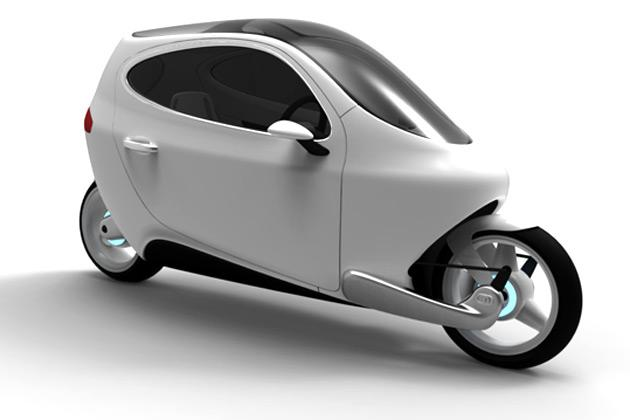
\includegraphics[width=0.4\linewidth]{fig1.png}
		\caption{Two-wheeled self-balancing car}
		\label{fig1}
	\end{figure} 
	
	The two-wheeled vehicle is composed of a cart system, a steering system (front part) and a body (rear part). Driven by the DC servo motor, the cart and steering systems allow drivers to change cart position and handle angle. To simplify the modeling in this mini-project, the self-balance two-wheeled vehicle is assumed to be stationary and the mechanical structure is given in Fig.~\ref{fig2}.
	
	\begin{figure}[htbp]
		\centering
		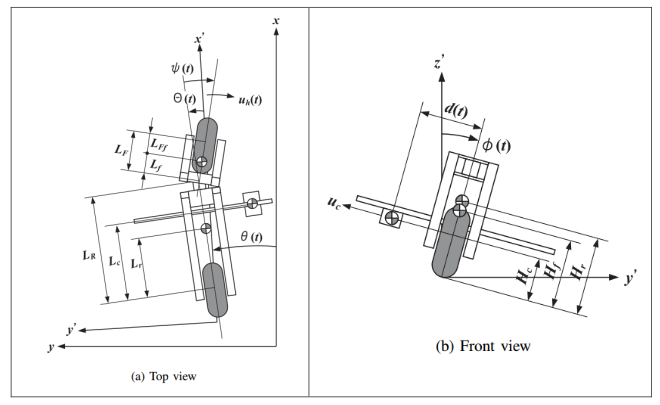
\includegraphics[width=0.6\linewidth]{fig2.png}
		\caption{Simple two-wheeled vehicle model}
		\label{fig2}
	\end{figure} 
	
	Then, state space model is established
	
	\begin{equation}
	\begin{split}
	\begin{aligned}
		\dot{x}&=Ax+Bu \\
		y&=Cx
	\label{eq1}
	\end{aligned}
	\end{split}
	\end{equation}
	
	where the state is designed according to the cart position, handle angle, bike angle and their corresponding velocities respectively
	
	\begin{equation}
		x=\begin{bmatrix}
		d(t) & \phi(t) & \psi(t) & \dot{d}(t) & \dot{\phi}(t) & \dot{\psi}(t) 
		\end{bmatrix}^{T}
	\label{eq2}
	\end{equation}
	
	and the relative matrices and input vectors are
	
	\begin{equation}
		A=\begin{bmatrix}
		0 &0  &0  &1  &0  &0 \\ 
		0 &0  &0  &0  &1  &0 \\ 
		0 &0  &0  &0  &0  &1 \\ 
		0 &6.5  &-10  &-\alpha   &0  &0 \\ 
		a_{51} &a_{52}  &a_{53}  &a_{54}  &a_{55}  &a_{56} \\ 
		5 &-3.6  &0  &0  &0  &-\gamma  
		\end{bmatrix}, 
		B=\begin{bmatrix}
		0 &0 \\ 
		0 &0 \\ 
		0 &0 \\ 
		\beta  &11.2 \\ 
		b_{51} &b_{52} \\ 
		40 &\delta  
		\end{bmatrix}
	\label{eq3}
	\end{equation}
	
	\begin{equation}
		C=\begin{bmatrix}
		1 &0  &0  &0  &0  &0 \\ 
		0 &1  &0  &0  &0  &0 \\ 
		0 &0  &1  &0  &0  &0 
		\end{bmatrix},
		D=\begin{bmatrix}
		u_{c}(t) &u_{h}(t) 
		\end{bmatrix}^{T}
	\label{eq4}
	\end{equation}
	
	The parameters in matrix $A$ and $B$ can be calculated as
	
	\begin{equation}
		%\begin{gather}
	\begin{split}
			a_{51}&=-\frac{M_{c}g}{den},
			a_{52}=\frac{(M_{f}H_{f}+M_{r}H_{r}+M_{c}H_{c})g}{den}, 
			a_{53}=\frac{(M_{r}L_{r}L_{F}+M_{c}L_{c}L_{F}+M_{f}L_{Ff}L_{R})g}{(L_{R}+L_{F})den}\\
			a_{54}&=-\frac{M_{c}H_{c}\alpha}{den},
			a_{55}=-\frac{\mu _{x}}{den},
			a_{56}=\frac{M_{f}H_{f}L_{Ff}\gamma }{den}\\		
			b_{51}&=\frac{M_{c}H_{c}\alpha }{den},
			b_{52}=-\frac{M_{f}H_{f}L_{Ff}\delta }{den},
			den=M_{f}H_{f}^{2}+M_{r}H_{r}^2+M_{c}H_{c}^{2}+J_{x}
			\label{eq5}			
		%\end{gather}
	\end{split}
	\end{equation}
	
	The physical parameters appering in Eq.~\ref{eq4} and Eq.~\ref{eq5} are usually measured mannually by experiments and they are given in appendix.
	
	After obtaining the linear system model and giving a step reference signal for each input channel, two basic response performance specifications are required to meet as follows
	
	\begin{itemize}
		\item The overshoot of system should below 10\%.
		\item The 2\% settling time should be less than 5 seconds.
	\end{itemize}

	The rest of the report is structured in the following manner: In section 2 a state feedback controller is designed using pole placement methods, followed by a discussion on effects of different pole choices. Section 3 concludes a Linear Quadratic Regulator controller design as well as the techique on choosing the weighting matrixes $Q$ and $R$. Section 4 introduces a state observer based on the former LQR control system and its performance is evaluated by monitoring the state estimation error. Section 5 describes a decoupling controller for a 2-input-2-output system. Section 6 designes a controller enabling the output of plant to track the reference signal regardless of step disturbances in input channel. Section 7 tries the integral control method to maintain outputs at a constatnt set point with zero steady-state error. Section 8 concludes the work.
	
	\section{State feedback controller by pole placement method}
	
	\subsection{Method description}
	
	\hspace{1.0em}
	Given the acquired six-order state space model, feedback controller is required to make the system stable. In this section, pole placement method will be used to obtain the feedback gain to meet control requirements. Firstly considering a second-order system, its overshoot and 2\% settling time of a step response is given as follows
	
	\begin{equation}
	M_{p}=e^{\frac{-\pi \zeta }{\sqrt{1-\zeta ^{2}}}}, t_{s}=\frac{4.0}{\zeta \omega _{n}}
	\label{eq6}
	\end{equation}
	
	where $\zeta$ and $\omega_{n}$ are damping ratio and natural frequency respectively. Now that the overshoot should below 10\% and settling time less than 5s, we set $\zeta=0.8$ and $\zeta\omega_{n}=2.5$ in this case, and then the two pole of second-order system is calculated as
	
	\begin{equation}
	\lambda _{1,2}=-\zeta \omega _{n}\pm j\omega _{n}\sqrt{1-\zeta ^{2}}
	\label{eq7}
	\end{equation}
	
	To assure the stability of system, the two dominant poles should have little smaller real parts, so we set them at $\lambda_{1,2}=-2.5\pm j1.875$. The other 4 poles are chosen 4-5 times lefter than the two dominant poles. Then the desired characteristic polynomial becomes
	
	\begin{equation}
	\begin{split}
	\begin{aligned}
		\phi _{d}(s)&=(s-\lambda _{1})(s-\lambda _{2})(s-\lambda _{3})(s-\lambda _{4})(s-\lambda _{5})(s-\lambda _{6})\\
		&=s^{6}+a_{5}s^{5}+a_{4}s^{4}+a_{3}s^{3}+a_{2}s^{2}+a_{1}s+a_{0}
	\end{aligned}
	\end{split}
	\label{eq8}
	\end{equation}
	
	The desired closed-loop matrix can be written in controllable canonical form
	
	\begin{equation}
	A_{d}=\begin{bmatrix}
	0 &  1&0  &0  &0  &0 \\ 
	0 &0  &1  &0  &0  &0 \\ 
	0 &0  &0  &1  &0  &0 \\ 
	0 &0  &0  &0  &1  &0 \\ 
	0 &0  &0  &0  &0  &1 \\ 
	-a_{5} &-a_{4}  &-a_{3}  & -a_{2} &-a_{1}  & -a_{0}
	\end{bmatrix}
	\label{eq9}
	\end{equation}
	
	Then the remainning task is transform the system with state feedback also to the controllable canonical form. First compute the controllability matrix and check if it is full rank
	
	\begin{equation}
	W_{c}=\begin{Bmatrix}
	B &AB  &A^{2}B  &A^{3}B &A^{4}B  & A^{5}B
	\end{Bmatrix}
	\label{eq10}
	\end{equation}
	
	Then select 6 independent vectors from $W_{c}$ in the strict order from left to right (the first six column vectors in this case) and group them in matrix X in the following form
	
	\begin{equation}
	X=\begin{Bmatrix}
	b_{1} &b_{2}  &Ab_{1}  &Ab_{2}  &A^{2}b_{1}  &A^{2}b_{2} 
	\end{Bmatrix}
	\label{eq11}
	\end{equation}
	
	Also compute the inverse of $X$ and write it as the following form
	
	\begin{equation}
	X^{-1}=\begin{bmatrix}
	q_{1}^{T} & q_{2}^{T} & q_{3}^{T} & q_{4}^{T} & q_{5}^{T} & q_{6}^{T}
	\end{bmatrix}^{T}
	\label{eq12}
	\end{equation}
	
	Because that the system has multiple input channels, choose the $3^{th} (d_{1}=3)$ and $6^{th} (d_{1}+d_{2}=6)$ row vectors of $X^{-1}$ and construct transformation matrix $T$ as
	
	\begin{equation}
	T=\begin{bmatrix}
	q_{3}^{T} &q_{3}^{T}A  &q_{3}^{T}A^{2}  & q_{6}^{T} &q_{6}^{T}A  &q_{6}^{T}A^{2}
	\end{bmatrix}^{T}
	\label{eq13}
	\end{equation}
	
	Define the feedback gain matrix $\bar{K}\in \mathbb{R}^{2\times 6}$ with 12 unknown variables, we can solve it by establishing the equation
	
	\begin{equation}
	\bar{A}-\bar{B}\bar{K}=A_{d}
	\label{eq14}
	\end{equation}
	
	where $\bar{A}=TAT^{-1}$, $\bar{B}=TB$
	
	After obtainning the matrix $\bar{K}$, we can finally get the original feedback gain matrix $K=\bar{K}T$. Substitute the control law $u=-Kx+r$ into Eq.~\ref{eq1} and the new closed-loop system becomes
	
	\begin{equation}
	\begin{split}
	\begin{aligned}
	\dot{x}&=(A-BK)x+Br \\
	y&=Cx
	\label{eq15}
	\end{aligned}
	\end{split}
	\end{equation}
	
	
	\subsection{Simulation results and refinements}
	
	\hspace{1.0em}
	In this report, the 6 poles are selected as $\lambda_{1,2}=-2.5\pm j1.875, \lambda_{3}=-10, \lambda_{4}=-10.75, \lambda_{5}=-11.5$ and $\lambda_{6}=-12.5$. The final feedback gain matrix $K$ is calculated to be
	
	\begin{equation}
	K=\begin{bmatrix}
	-15.68 &12.20  &6.27  &4.90  &-6.21  &-2.26 \\ 
	250960 &-21110  &-107660  &-845.58  &9043.2  &412.98 
	\end{bmatrix}
	\nonumber
	\end{equation}
	
	The number of elements differes a lot and are relatively weird. Temporarily we use the feedback matrix and simulate the closed-loop system with time domain from 0 to 10 seconds. Given a step signal for each input channel, the output response is showed in Fig.~\ref{fig3}. Sadly though the system becomes stable with a short settling time, there are huge overshoots in both cases and the stable points are also impossible in real cases. 
	
	\begin{figure}[htbp]
		\centering
		\begin{minipage}[t]{0.48\textwidth}
			\centering
			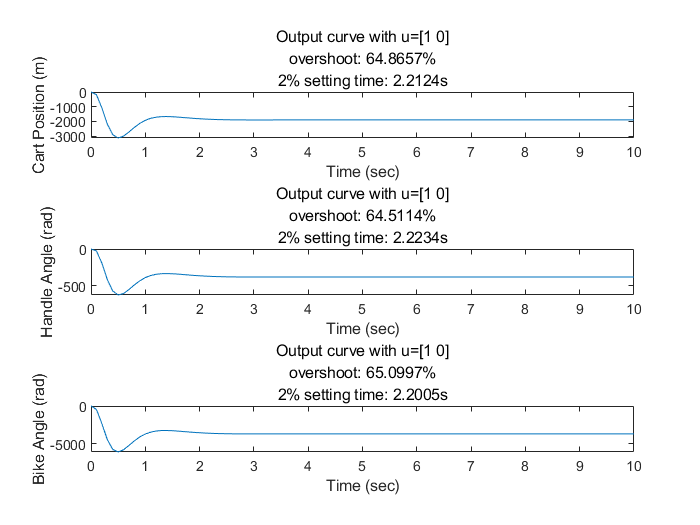
\includegraphics[width=8cm]{fig3.png}
		\end{minipage}
		\begin{minipage}[t]{0.48\textwidth}
			\centering
			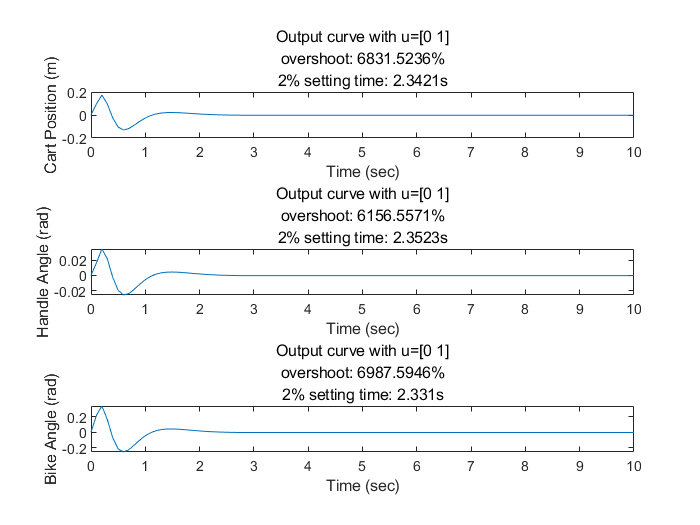
\includegraphics[width=8cm]{fig4.png}
		\end{minipage}
	\caption{Step response for the closed-loop system}
	\label{fig3}
	\end{figure}
	
	The results are unacceptable and need further refinements. Obviously, the bad results are closely realted to the feedback gain matrix $K$, which influnces the system matrix $A-BK$ of closed-loop system. In another point of view, we can find infinite $K$ to place the same poles for a plant as there are infinite system matrixes with the same eigenvalues. 
	
	Actuallly when tackling pole placement problems for high order system, some pole choices will result in sensitivity problems, which leads to a large gain as in our former method. One robust algorithm was proposed in \cite{kautsky1985robust} and has been applied in matlab function. The aim of this algorithm is to find the feedback gain matrix $K$ that makes $A-BK$ the most robust. One method to measure the robustness of a matrix is to use condition number
	
	\begin{equation}
	c_{j}=\frac{1}{s_{j}}=\frac{\left \| y_{j} \right \|_{2} \left \| x_{j} \right \|_{2}}{\left |y_{j}^{T} x_{j}  \right |}
	\label{eq16}
	\end{equation}
	
	where $x_{j}$ and $y_{j}$ are the left and right eigenvalues of $A-BK$ respectively. It can be proved that $c_{j}$ has a upper bound i.e. $max_{j}c_{j} \leq \kappa _{2}(X)\equiv \left \| X \right \|_{2}\left \| X^{-1} \right \|_{2}$, where $X=\begin{bmatrix}
	x_{1} &x_{2}  &\cdots   & x_{n}
	\end{bmatrix}$ is the eigenvector matrix. The maximum value $v=max(c_{j})$ of all condition numbers is chosen and the system is said to be the most robust if $v$ is the smallest. Then the problem becomes how to find the minimum upper bound of condition numbers.
	
	The minimum upper bound can ben found by cauchy inequality and the result is given as follows
	
	\begin{equation}
	min ( \kappa _{2}(X)) \leq \frac{\kappa _{2}(S)}{\sqrt{k}}
	\label{eq17}
	\end{equation}
	
	$S$ is orthogonal normal basis of the null space of $N(U_{1}^{T}(A-\lambda I))$, where $U_{1}$ is the orthogonal basis of null space of input matrix $B$, $\lambda$ are eigenvalues of matrix $A-BK$ and $k$ is the dimensions of $S$. QR decomposition or singular value decomposition (SVD) can be used to calculate the orthogonal basis. Finally, feedback gain matrix $K$ can be obtained by
	
	\begin{equation}
	K=Z^{-1}U_{0}^{T}(A-X\Lambda X^{-1})
	\label{eq18}
	\end{equation}
	
	where $\Lambda=diag(\lambda_{1},\lambda_{2},...,\lambda_{n})$, $Z$ is the $Q$ matrix of $B$ and $U_{0}$ is also orthogonal basis of $B$.
	
	The same poles are chosen but we use the new method to calculate feedback matrix ${K}'$, the result is given below
	
	\begin{equation}
	{K}'=\begin{bmatrix}
	8.7165 &-3.6746  &-1.8207  &0.5685  &-0.4985  &-0.0880 \\ 
	-11.2971 &10.6474  &5.4543  &-0.8739  &1.4368  &0.3794 
	\end{bmatrix}
	\nonumber
	\end{equation}
	
	The step response for the new closed-loop system is shown in Fig.~\ref{fig4} and both the overshoot and settling time meet the requirements. Now assume that all six states can be observed, their response with non-zero initial condition $x_{0}$ to zero external inputs is given in Fig.~\ref{fig5}. It is clearly shown that all states are stable and no weired values apper.
	
	\begin{figure}[htbp]
		\centering
		\begin{minipage}[t]{0.48\textwidth}
			\centering
			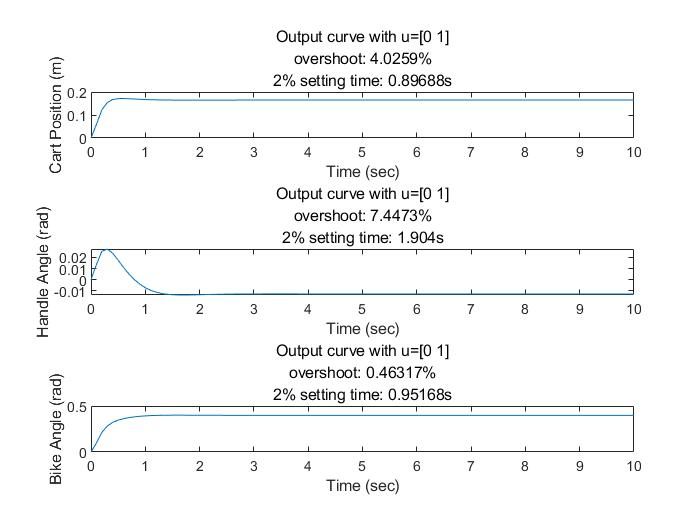
\includegraphics[width=8cm]{fig5.png}
		\end{minipage}
		\begin{minipage}[t]{0.48\textwidth}
			\centering
			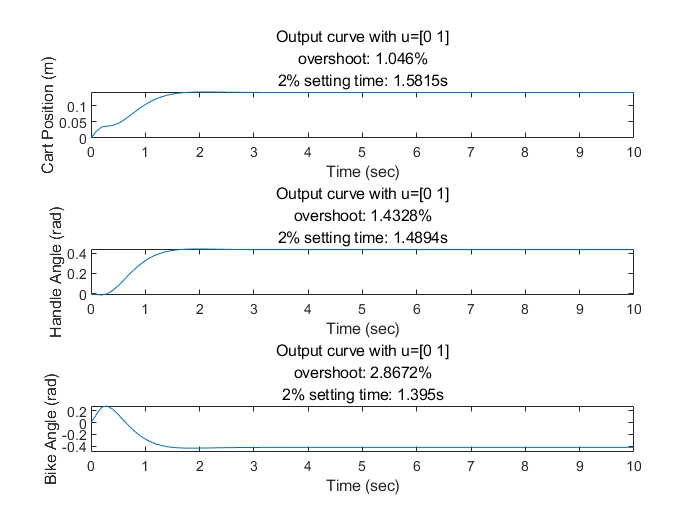
\includegraphics[width=8cm]{fig6.png}
		\end{minipage}
		\caption{Step response for the new closed-loop system}
		\label{fig4}
	\end{figure}

	\begin{figure}[htbp]
		\centering
		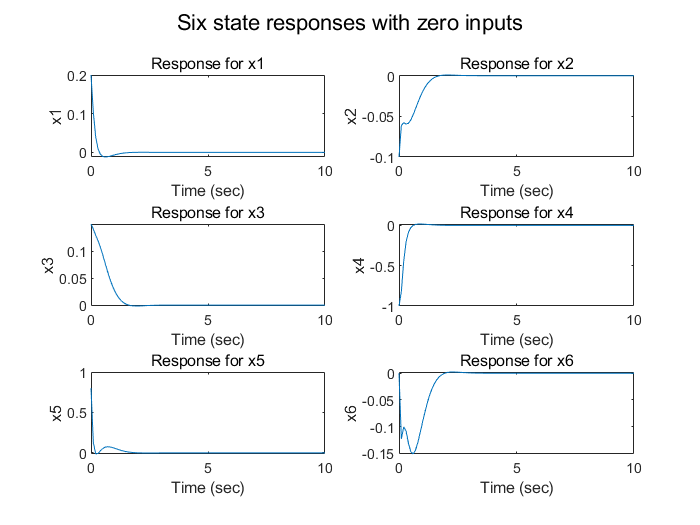
\includegraphics[width=0.8\linewidth]{fig7.png}
		\caption{All state responses with zero inputs}
		\label{fig5}
	\end{figure} 
	
	\subsection{Discussion}
	
	\hspace{1.0em}
	With refinements on feedback gain matrix $K$, the overshoot of the closed-loop system is largely cut down as well as its sensitivity to noise. On the other side, the system performance is also largely affected by different pole choosing strategies. Although one can always stablize the system and make system response faster by designing poles on the very left plain, the input cost will increase in this case. To investigate the influence of poles, two more groups of poles are used. The new poles are listed as followings
	
	\begin{equation}
	\begin{split}
	\begin{aligned}
	{p}'&= \begin{bmatrix}
	-1.6+j0.96 &-1.6-j0.96  &-6.4  &-6.88  &-7.36  &-8
	\end{bmatrix}\\
	{p}''&= \begin{bmatrix}
	-4+j3 &-4-j3  &-16  &-17.2  &-18.4  &-20 
	\end{bmatrix}
	\end{aligned}
	\end{split}
	\nonumber
	\end{equation}
	
	It is clearly shown in Fig.~\ref{fig6}, \ref{fig7} and \ref{fig8} that the larger negative real parts the pole has, the more control effect is required. However if the designed poles are too right, large overshoot or long settling time may be expected to appear (as is shown in Fig.~\ref{fig9}).
	
	\begin{figure*}[htbp] %通栏
		\begin{minipage}[t]{0.33\linewidth} %调节两个子图左右间距
			\centering
			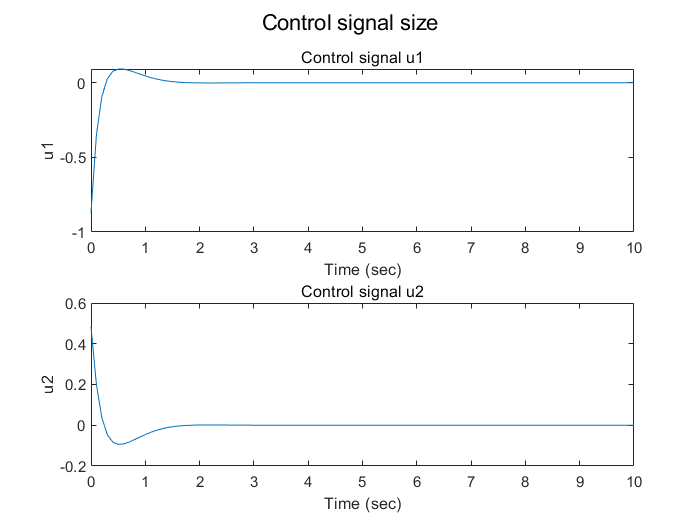
\includegraphics[width=2.4in, height=1.9in]{fig8.png} %调节单个子图大小
			\caption{Control signal size with $p$} %子图下标题
			\label{fig6}
		\end{minipage}%
		\begin{minipage}[t]{0.33\linewidth}
			\centering
			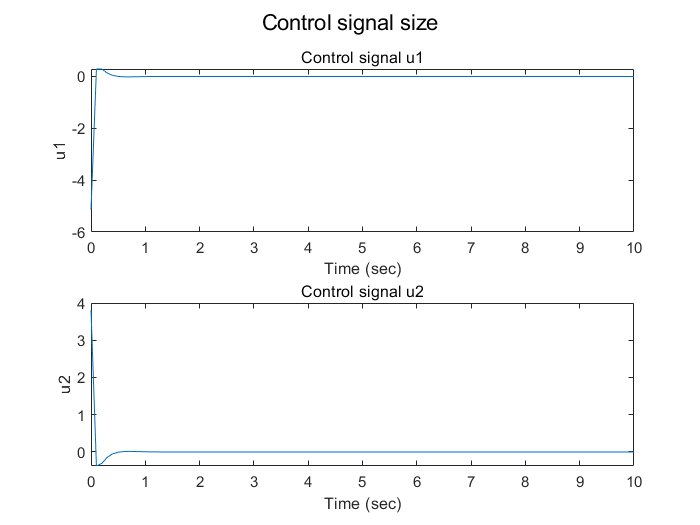
\includegraphics[width=2.4in, height=1.9in]{fig9.png}
			\caption{Control signal size with ${p}'$}
			\label{fig7}
		\end{minipage}%
		\begin{minipage}[t]{0.33\linewidth}
			\centering
			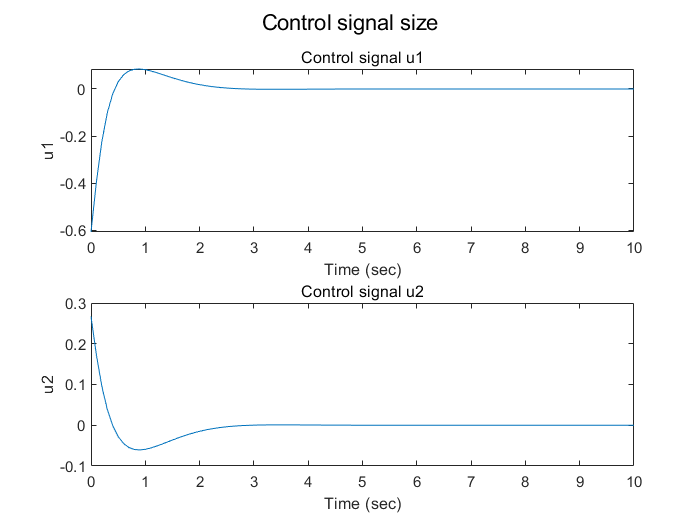
\includegraphics[width=2.4in, height=1.9in]{fig10.png}
			\caption{Control signal size with ${p}''$}
			\label{fig8}
		\end{minipage}
	\end{figure*}

	\begin{figure}[htbp]
		\centering
		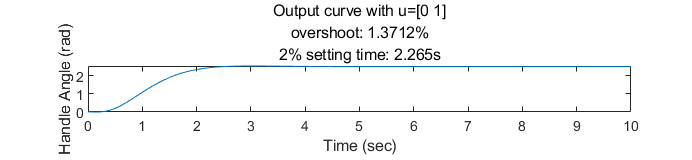
\includegraphics[width=0.6\linewidth]{fig11.png}
		\caption{Large overshoot show when given ${p}''$ with small negative real parts}
		\label{fig9}
	\end{figure}
	
	Pole placement methods have the magic of easily stabilizing the system and ensuring the expected design performance by using state feedback controller. On the other hand, poles of systems are hard to select and have no strict standards. In next section, linear quadratic regulator will be introduced to solve the trade-off problem between system performance and control cost.
	
	
	\section{Linear quadratic regulator controller}
	
	\subsection{Method description}
	
	\subsubsection{Class method}
	
	\hspace{1.0em}
	Linear quadratic resgulator (LQR) follows the theory of optimal control, which is aimed to minimized the cost function. Given a multi-input-multi-output system and consider both control performance and input cost, the cost function can be defined as
	
	\begin{equation}
	J=\frac{1}{2}\int_{0}^{\infty}(x^{T}Qx+u^{T}Ru)dt
	\label{eq19}
	\end{equation}
	
	The $Q$ and $R$ in Eq.~\ref{eq19} are weighting matrixes representing cost on response speed and energy efficiency respectively. After selecting the appropriate weighting matrix, a state feedback controller $u=-Kx+r$ can be designed to minimize the cost function, where the gain matrix $K=R^{-1}B^{T}P$ and matrix $P$ is given by solving the Riccati equation
	
	\begin{equation}
	A^{T}P+PA+Q-PBR^{-1}B^{T}P=0
	\label{eq20}
	\end{equation}
	
	Then the problem becomes solving the algebraic matrix riccati equation. One method is to use an eigenvalue-eigenvector based algorithm. First a $2n \times 2n$ matrix is derived
	
	\begin{equation}
	\Gamma =\begin{bmatrix}
	A &-BR^{-1}B^{T} \\ 
	-Q &-A^{T} 
	\end{bmatrix}
	\label{eq21}
	\end{equation}
	
	Then $n$ stable eigenvalues of $\Gamma$ are found as well as their corresponding eigenvectors. Write the eigenvectors in the form of $\begin{pmatrix}
	v_{i} & u_{i}
	\end{pmatrix}^{T},i=1,2,\cdots ,n$. Then the $P$ matrix in riccati equation can be calculated by
	
	\begin{equation}
	P=\begin{pmatrix}
	\mu _{1} &\cdots   & \mu _{n}
	\end{pmatrix}
	\begin{pmatrix}
	v_{1} &\cdots   & v_{n}
	\end{pmatrix}^{-1}
	\label{eq22}
	\end{equation}
	
	\subsubsection{Discrete LQR method}
	
	\hspace{1.0em}
	Another method is given by considering a discrete case. Similarly, a discrete cost function is given in Eq.~\ref{eq23}.
	
	\begin{equation}
	J=\frac{1}{2}\sum_{k=0}^{\infty}(x_{k}^{T}Qx_{k}+u_{k}^{T}Ru_{k})
	\label{eq23}
	\end{equation}
	
	The first step is to discretize the state space equation. According to the mean value theorem of integral
	
	\begin{equation}
	x(t+dt)=x(t)+Ax(\xi )dt, \xi \in (t,t+dt)
	\label{eq24}
	\end{equation}
	
	where $dt$ is the dicrete time interval set mannually. Here we use midpoint euler method ($x(\xi)=\frac{x(t)+x(t+dt)}{2}$) to estimate the next state, we got
	
	\begin{equation}
	x(t+dt)=(I-\frac{Adt}{2})^{-1}(I+\frac{Adt}{2})x(t)
	\label{eq25}
	\end{equation}
	
	Back to the state space equation in Eq.~\ref{eq1}, we integrate both sides and get
	
	\begin{equation}
	\int_{t}^{t+dt}\dot{x}=\int_{t}^{t+dt}(Ax+Bu)dt\Rightarrow x(t+dt)-x(t)=Ax(\xi )dt+Bu(\xi)dt
	\label{eq26}
	\end{equation}
	
	By substituting Eq.~\ref{eq25} into it and take some approximation, we finally get
	
	\begin{equation}
	x(t+dt)=(I-\frac{Adt}{2})^{-1}(I+\frac{Adt}{2})x(t)+Bdtu(t)
	\label{eq27}
	\end{equation}
	
	Now we can rewrite Eq.~\ref{eq27} into a form of dicrete state space model
	
	\begin{equation}
	x(k+1)=\bar{A}x(k)+\bar{B}u(k)
	\label{eq28}
	\end{equation}
	
	where $\bar{A}=(I-\frac{Adt}{2})^{-1}(I+\frac{Adt}{2})$ and $\bar{B}=Bdt$.
	
	The second step is to solve the discrete riccati equation
	
	\begin{equation}
	P=Q+\bar{A}^{T}P\bar{A}-\bar{A}^{T}P\bar{B}(R+\bar{B}^{T}P\bar{B})^{-1}\bar{B}^{T}P\bar{A}
	\label{eq29}
	\end{equation}
	
	$P$ can be solved numerically by iteration method. Usually we give $P$ a initial value as $Q$ and $P$ will quickly converges after a number of iterations. With the matrix $P$, we finally get the feedback gain matrix $K=(R+\bar{B}^{T}P\bar{B})^{-1}\bar{B}^{T}P\bar{A}$.
	
	
	\subsection{Simulation results}
	
	\hspace{1.0em}
	Like what we did in Section 1, we first evaluate the closed-loop system performance under a step signal input for each channel with zero initial conditions. Since we obtain two methods for LQR controller, a comparison between them (with the same weighting matrix $Q$ and $R$) is also given.
	
	We initially select weighting matrix $Q=diag\begin{Bmatrix}
	10 &50  &50  &5  &50  &50 
	\end{Bmatrix}$ and $R=I_{6\times 6}$. With the first eigenvalue-based method, the feedback gain matrix $K$ is acquired as
	
	\begin{equation}
	K=\begin{pmatrix}
	54.3246 &-45.5065  &-19.2405  &5.2022  &-5.3849  &2.3616 \\ 
	-45.7713 &39.8256  &25.5740  &-4.0248  &5.4445  &6.9241 
	\end{pmatrix}
	\nonumber
	\end{equation}
	
	Then the closed-loop system is simulated as is shown in Fig.~\ref{fig10}. The system is stabilized and successfully meet the design specifications. With the selected weighting matrix $Q$ and $R$, there exists no overshoot and the settling time are all around 4s.
		
	\begin{figure}[htbp]
		\centering
		\begin{minipage}[t]{0.48\textwidth}
			\centering
			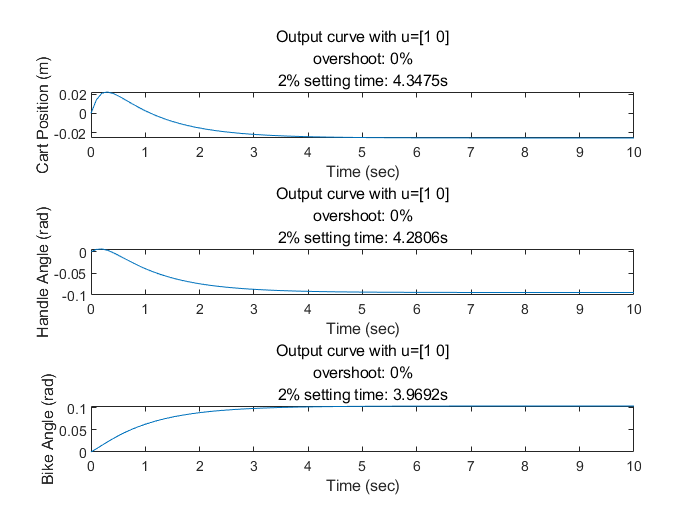
\includegraphics[width=8cm]{fig12.png}
		\end{minipage}
		\begin{minipage}[t]{0.48\textwidth}
			\centering
			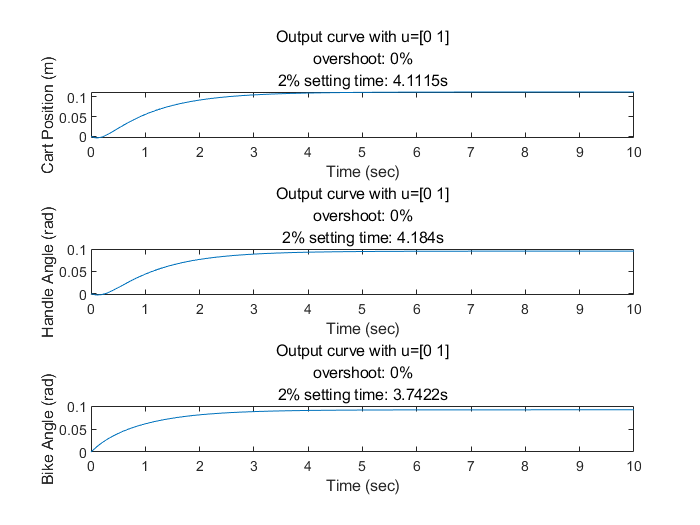
\includegraphics[width=8cm]{fig13.png}
		\end{minipage}
		\caption{Step response for closed-loop system by eigenvalue-based LQR method}
		\label{fig10}
	\end{figure}
	
	Then the second discrete LQR method is applied. We suppose that the matrix $P$ converges when the mean of elements in $\mid P_{new}-P_{old} \mid$ is less than a small number. The gain matrix $K$ is calculated as
	
	\begin{equation}
	K=\begin{pmatrix}
	46.7765 &-39.2025  &-19.5779  &4.2947  &-4.8494  &-0.6493 \\ 
	-33.3206 &28.1860  &15.6346  &-3.0081  &3.6233  &1.9127 
	\end{pmatrix}
	\nonumber
	\end{equation}
	
	The simulation results is shown in Fig.~\ref{fig11}. Compared with the eigenvalue-based one, this discrete lqr method have a little more overshoot but also cut down the settling time in most cases. The dlqr method is also computationally efficient because the matrix $P$ will quickly converges while the first method always need to handle the eigenvalue problem. However, when step signal is added in first input channel, the settling time is over 5s and unable to meet the basic design specifications. Therefore we will still use the eigenvalue-based method in the following discussion.
	
	\begin{figure}[htbp]
		\centering
		\begin{minipage}[t]{0.48\textwidth}
			\centering
			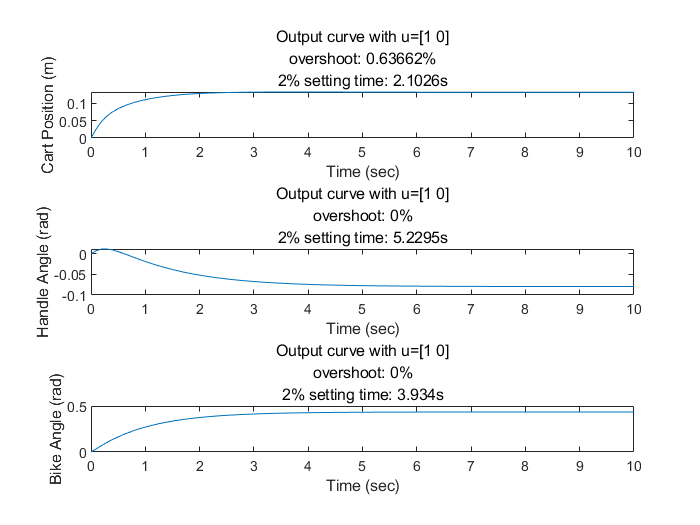
\includegraphics[width=8cm]{fig15.png}
		\end{minipage}
		\begin{minipage}[t]{0.48\textwidth}
			\centering
			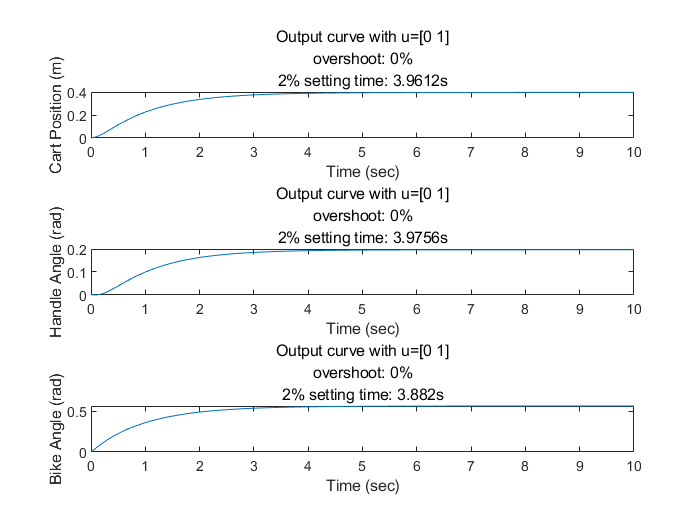
\includegraphics[width=8cm]{fig14.png}
		\end{minipage}
		\caption{Step response for closed-loop system by discrete LQR method}
		\label{fig11}
	\end{figure}

	Fig.~\ref{fig12} also gives the six state responses to non-zero initial state condition $x_{0}$ with zero external inputs. All states becomes stable at zero point in a short time as expected.
	
	\begin{figure}[htbp]
		\centering
		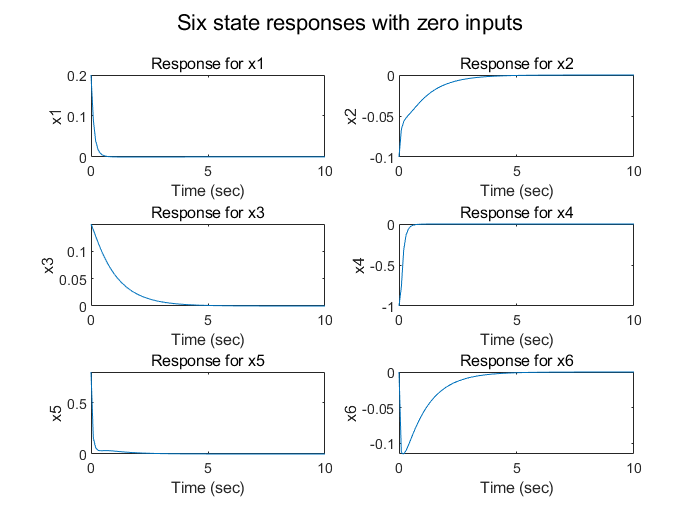
\includegraphics[width=0.6\linewidth]{fig16.png}
		\caption{State response with zero external inputs}
		\label{fig12}
	\end{figure}
	
	\subsection{Discussion}
	
	\hspace{1.0em}
	Rather than design poles to stabilize the system, LQR method achieves the stability by choosing reasonable weighting matrix $Q$ and $R$. To investigate their effects on system, we remain $R$ unchanged and multiply the $Q$ matrix with a scalar to form ${Q}'=\begin{Bmatrix}
	5&  25&  25&  2.5&  25& 25
	\end{Bmatrix}$. By monitoring the control signal cost and comparing it with the original system (Fig.~\ref{fig13}), we can find that with a smaller $Q$, the energy cost is reduced. We also keep $Q$ unchanged and design a new $R$ matrix with bigger weights. The simulation results is given in Fig.~\ref{fig14}, where the bigger $R$ gives a greater punishment on control energy and LQR controller automatically cut down the control signal.
	
	\begin{figure}[H]
		\centering
		\begin{minipage}[t]{0.48\textwidth}
			\centering
			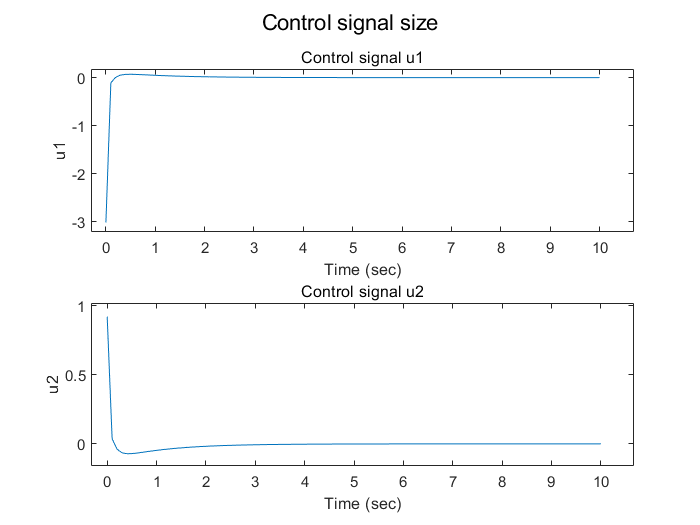
\includegraphics[width=8cm]{fig17.png}
		\end{minipage}
		\begin{minipage}[t]{0.48\textwidth}
			\centering
			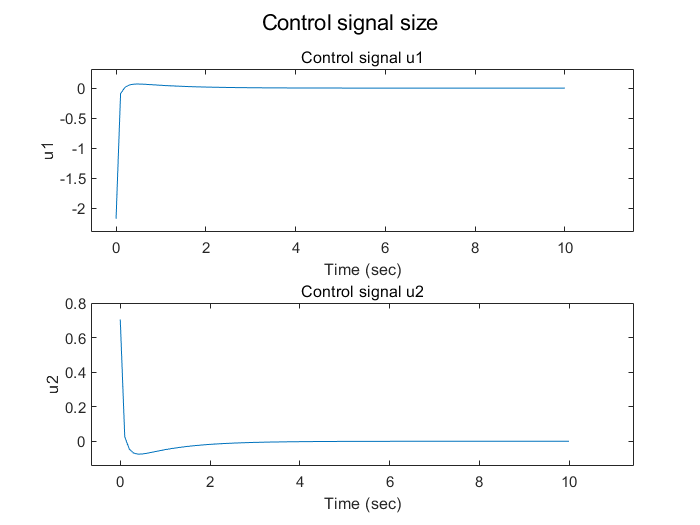
\includegraphics[width=8cm]{fig18.png}
		\end{minipage}
		\caption{Comparison between control cost with $Q$ and ${Q}'$ ($R$ remain unchanged)}
		\label{fig13}
		
		\begin{minipage}[t]{0.48\textwidth}
			\centering
			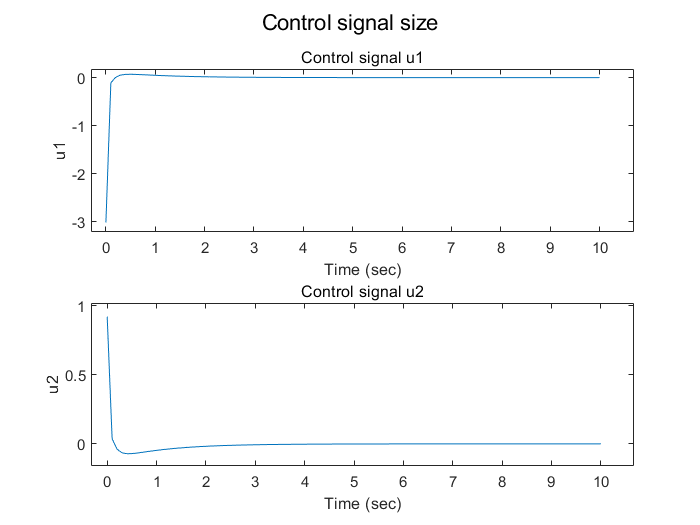
\includegraphics[width=8cm]{fig17.png}
		\end{minipage}
		\begin{minipage}[t]{0.48\textwidth}
			\centering
			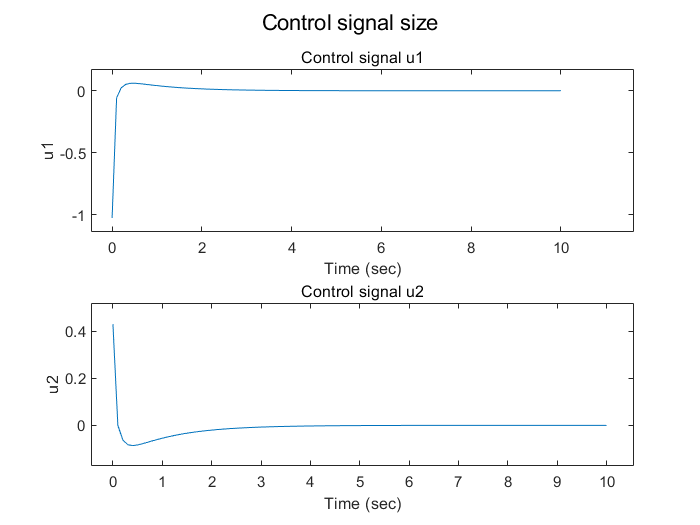
\includegraphics[width=8cm]{fig19.png}
		\end{minipage}
		\caption{Comparison between control cost with $R$ and ${R}'$ ($Q$ remain unchanged)}
		
		\label{fig14}
	\end{figure}

	Similar with the pole placement methods, LQR controller offers a way to do trade-off between response speed and control signal cost by tuning the weighting matrixes. In practical situation, one can define the most reasonable cost function according to the established mathematic model. Unlike selecting poles by experience and check system performance repeatedly, LQR method can always find the optimal solution as long as the cost function is given.
	
	\section{Observer-based LQR control system}
	
	\subsection{Method description}
	
	\hspace{1.0em}
	In practice, not all state variables can be measured for a system and an observer is required to estimate these unseen states. Suppose the estimated state is $\hat{x}(t)$ and the true state is $x(t)$, then the state estimate error is
	
	\begin{equation}
	\tilde{x}(t)=x(t)-\hat{x}(t)
	\label{eq30}
	\end{equation}
	
	We hope the error dynamics is adjustable and converges to zero with time, thus a closed-loop estimator is used (Fig.~\ref{fig15}).
	
	\begin{figure}[htbp]
		\centering
		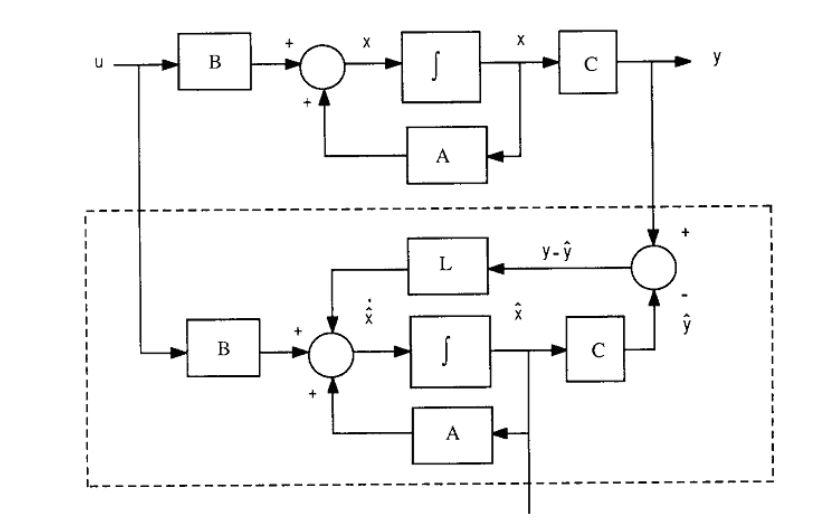
\includegraphics[width=0.6\linewidth]{fig20.png}
		\caption{A closed-loop estimator}
		\label{fig15}
	\end{figure}

	The state space equation for estimator is derived in Eq.~\ref{eq31} and also the state estimation error in Eq.~\ref{eq32}.
	
	\begin{equation}
	\dot{\hat{x}}(t)=A\hat{x}(t)+Bu(t)+L(y-C\hat{x})
	\label{eq31}
	\end{equation}
	
	\begin{equation}
	\dot{\tilde{x}}(t)=(A-LC)\tilde{x}
	\label{eq32}
	\end{equation}
	
	Then observer poles can be selected to get the observer gain matrix $L$ using pole placement algorithms. Remember in early sections we simply use the invisible state variables to design the state feedback controller, which is unpractical in actual situations. Now we can implement the estimated state $\hat{x}$ in our LQR controller and evaluate the new closed-loop system. Consider the control law $u=-K\hat{x}+r$ and substitute it into the original state space equation, and also combine with Eq.~\ref{eq32} to form a new system
		
	\begin{equation}
	\begin{split}
	\begin{aligned}
		\begin{bmatrix}
		\dot{x}\\ \dot{\tilde{x}}
		\end{bmatrix}&=\begin{bmatrix}
		A-BK &BK \\ 
		0 &A-LC 
		\end{bmatrix}
		\begin{bmatrix}
		x\\\tilde{x} 
		\end{bmatrix}+
		\begin{bmatrix}
		B\\0 	
		\end{bmatrix}r
		\\
		y&=Cx
	\label{eq33}
	\end{aligned}
	\end{split}
	\end{equation}
	
	From Eq.~\ref{eq33}, we can deduce the Laplace transform of the combined system
	
	\begin{gather}
%	\begin{equation}
%	\begin{split}
	X(s)=(sI-A+BK)^{-1}x(0)+(sI-A+BK)^{-1}BK(sI-A+LC)^{-1}\tilde{x}(0)+(sI-A+BK)^{-1}BR(s) \nonumber\\
	\tilde{X}(s)=(sI-A+LC)^{-1}\tilde{x}(0)
	\label{eq34}
%	\end{split}
%	\end{equation}
	\end{gather}
	
	It is clear that there would be no state estimation error if the initial estimated state is the same with real one ($\tilde{x}(0)=0$). Now that we couldn't acquire the real $x(0)$ in most cases, we assume our initial estimated $\hat{x}(0)$ to be zero.
	
	
	\subsection{Simulation results and discussion}
	
	\hspace{1.0em}
	First we select observer poles 3 times faster than the control poles $p$ used in section 1. Also we modeify the $Q$ and $R$ in LQR controller to achieve a better system performance. The new weighting matrix are $Q=diag\begin{Bmatrix}
	4&  22&  22&  4&  22&22 
	\end{Bmatrix}$ and $R=5I$ respectively. The system's zero-state response with a step signal in each channel is given in Fig.~\ref{fig16}. The six responses all have small overshoots and are stabilize with time, but in the left picture the settling time for the first ouput channel is a little bit longer. We can plot the state estimation error with time in Fig.~\ref{fig17}, where all of the errors quickly converges to zero in 1s.
	
	\begin{figure}[H]
		\centering
		\begin{minipage}[t]{0.48\textwidth}
			\centering
			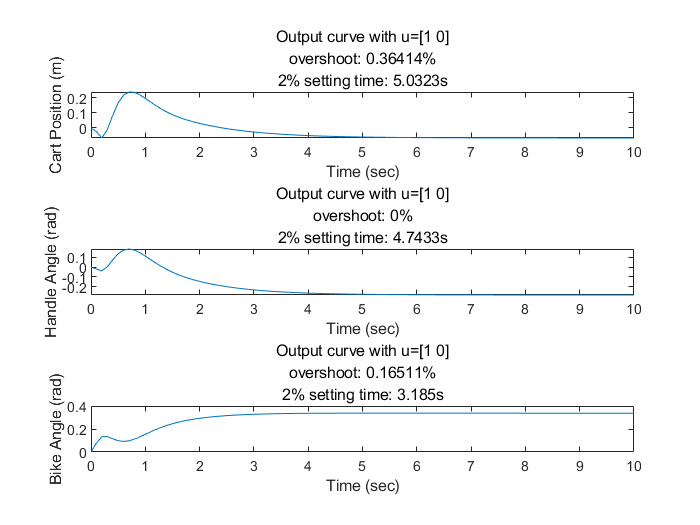
\includegraphics[width=8cm]{fig22.png}
		\end{minipage}
		\begin{minipage}[t]{0.48\textwidth}
			\centering
			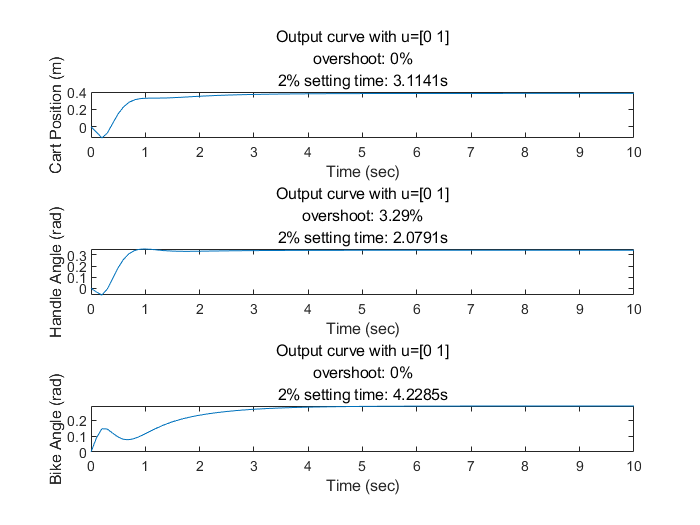
\includegraphics[width=8cm]{fig21.png}
		\end{minipage}
		\caption{Step response for the observed-based system}
		\label{fig16}
	\end{figure}

	\begin{figure}[H]
		\centering
		\begin{minipage}[t]{0.48\textwidth}
			\centering
			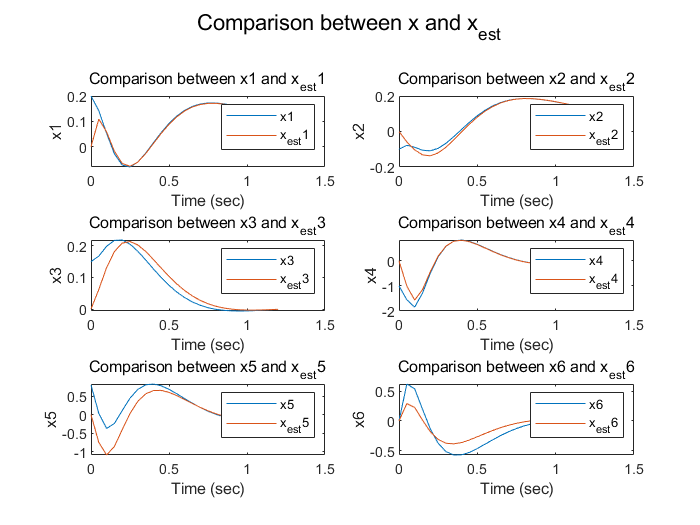
\includegraphics[width=8cm]{fig23.png}
		\end{minipage}
		\begin{minipage}[t]{0.48\textwidth}
			\centering
			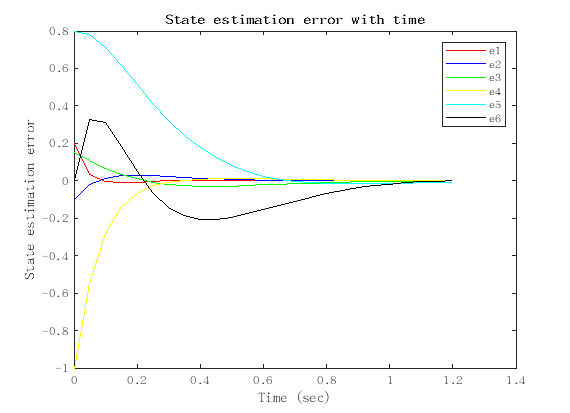
\includegraphics[width=8cm]{fig24.png}
		\end{minipage}
		\caption{Investigation on state estimation error}
		\label{fig17}
	\end{figure}
	
	Then we keep weighting matrixes unchanged and modify the observer poles. Two new pairs of poles are selected as 2 and 4 times faster than the control poles. The simulation results are illustrated in Fig.~\ref{fig18} and Fig.~\ref{fig19}. We can see that in when the observer poles are too left, overshoots are largely increased while settling time are almost unchanged in both cases.
	
	\begin{figure}[H]
		\centering
		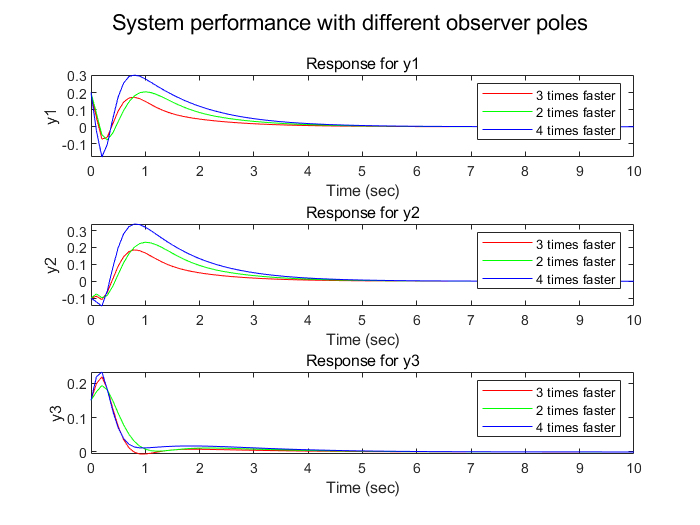
\includegraphics[width=0.6\linewidth]{fig25.png}
		\caption{Comparison of system performance with different observer poles (zero input, non-zero condition)}
		\label{fig18}
	\end{figure}

	The state estimation error with these two different pairs of poles are given in Fig.~\ref{fig19} and Fig.~\ref{fig20}. It is clearly shown the state estimation error converges to zero faster with observer poles on the more left plain. However, large overshoots may also appear at the same time. 

	\begin{figure}[H]
		\centering
		\begin{minipage}[t]{0.48\textwidth}
			\centering
			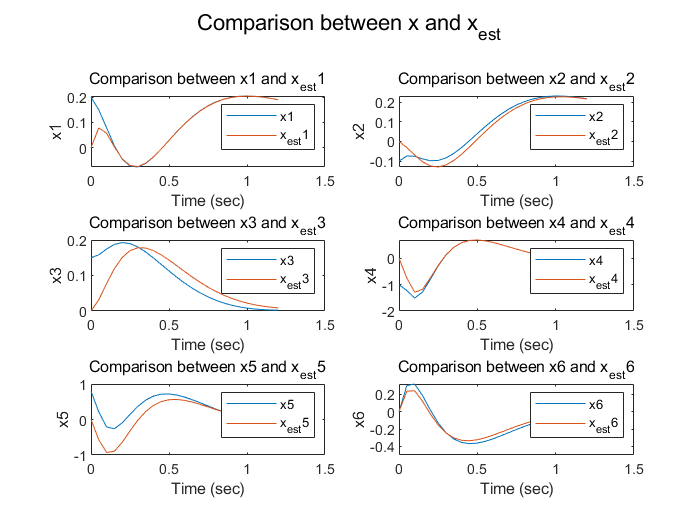
\includegraphics[width=8cm]{fig26.png}
		\end{minipage}
		\begin{minipage}[t]{0.48\textwidth}
			\centering
			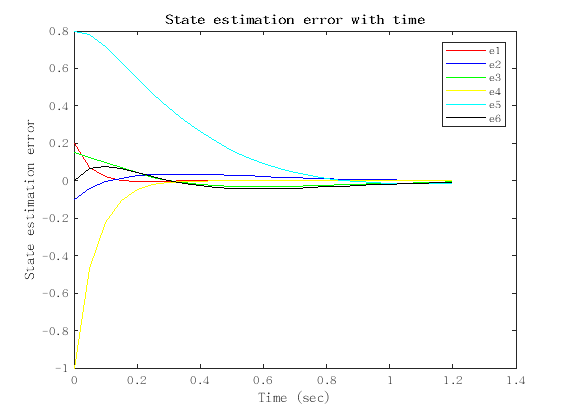
\includegraphics[width=8cm]{fig27.png}
		\end{minipage}
		\caption{State estimation error with slower observer poles}
		\label{fig19}
	\end{figure}
	
	\begin{figure}[H]
		\centering
		\begin{minipage}[t]{0.48\textwidth}
			\centering
			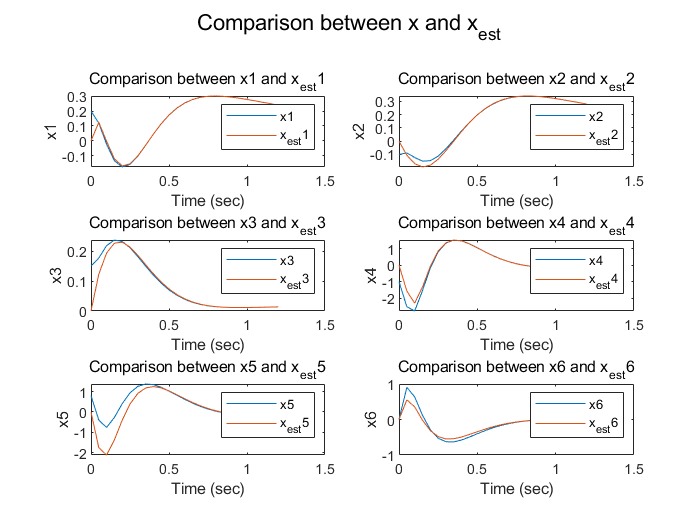
\includegraphics[width=8cm]{fig28.png}
		\end{minipage}
		\begin{minipage}[t]{0.48\textwidth}
			\centering
			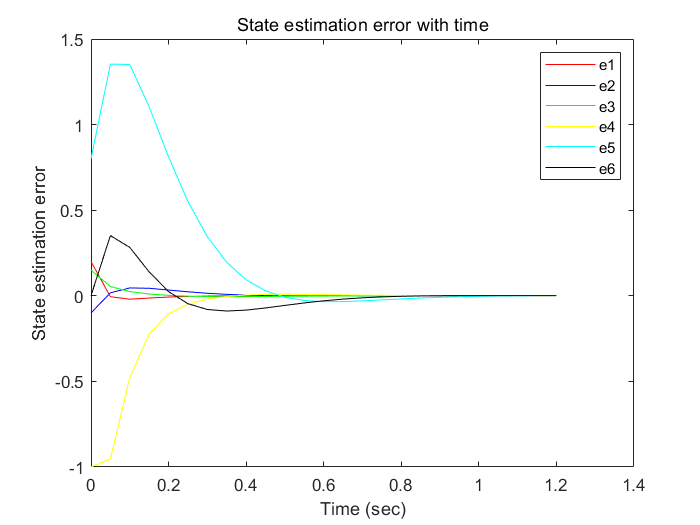
\includegraphics[width=8cm]{fig29.png}
		\end{minipage}
		\caption{State estimation error with faster observer poles}
		\label{fig20}
	\end{figure}
	
	\section{System decoupling control}
	
	\subsection{Method description}
	
	\subsubsection{Decoupling by state feedback}
	
	\hspace{1.0em}
	In this section, we suppose that cart position $d(t)$ and bike angle $\psi (t)$ are the most two interesting outputs and the new output matrix is
	
	\begin{equation}
	C_{2}=\begin{bmatrix}
	1 &0  &0  &0  &0  &0 \\ 
	0 &0  &1  &0  &0  &0 
	\end{bmatrix}
	\label{eq35}
	\end{equation}
	
	Then the plant becomes a 2-input-2-output system. To achieve decoupling control, a state feedback control law $u=-Kx+Fr$ is applied such that 
	
	\begin{equation}
	\begin{split}
	\begin{pmatrix}
	y_{1}(s)\\y_{2}(s) 
	\end{pmatrix}=\begin{pmatrix}
	h_{11} &0 \\ 
	0 &h_{22} 
	\end{pmatrix}\begin{pmatrix}
	r_{1}(s)\\ 
	r_{2}(s)
	\end{pmatrix}
	\end{split}
	\label{eq36}
	\end{equation}
	
	The closed-loop state space system becomes $\dot{x}=(A-BK)x+BFu$, and by laplace tranformation, we can relate the open-loop and closed loop transfer function matrix:
	
	\begin{equation}
	H(s)=G(s)[I+K(sI-A)^{-1}B]^{-1}F
	\label{eq37}
	\end{equation}
	
	where $G(s)=C(sI-A)^{-1}B$.
	
	To decouple the system we need $H(s)$ to be diagonal and thus $G(s)$ should be non-singular. It can be proved that $G(s)$ can be written in the form of
	
	\begin{equation}
	G(s)=\begin{pmatrix}
	g_{1}^{T}(s)\\ 
	g_{2}^{T}(s)\\ 
	\vdots \\ 
	g_{m}^{T}(s)
	\end{pmatrix}=\begin{pmatrix}
	s^{-\sigma _{1}} &0  &\cdots   &0 \\ 
	0 &s^{-\sigma _{2}}  &\cdots   &0 \\ 
	\vdots  &\vdots   &\ddots   &\vdots  \\ 
	0 &0  &\cdots   &s^{-\sigma _{m}} 
	\end{pmatrix}[B^{*}+C^{*}(sI-A)^{-1}B]
	\label{eq38}
	\end{equation}
	
	where $B^{*}=\begin{pmatrix}
	c_{1}^{T}A^{\sigma _{1}-1}B\\ 
	c_{2}^{T}A^{\sigma _{2}-1}B\\ 
	\vdots \\ 
	c_{m}^{T}A^{\sigma _{m}-1}B
	\end{pmatrix},
	C^{*}=\begin{pmatrix}
	c_{1}^{T}A^{\sigma _{1}}\\ 
	c_{2}^{T}A^{\sigma _{2}}\\ 
	\vdots \\ 
	c_{m}^{T}A^{\sigma _{m}}
	\end{pmatrix}$ and the relative degree $\sigma_{i}$ can be derived by Eq.~\ref{eq39} 
	
	\begin{equation}
	\sigma _{i}=\left\{\begin{matrix}
	min(j|c_{i}^{T}A^{i-1}B\neq 0^{T}, j=1,2,\cdots ,n  )\\ 
	n,\quad if \quad c_{i}^{T}A^{i-1}B=0^{T} \quad i=1,2,\cdots ,n
	\end{matrix}\right.
	\label{eq39}
	\end{equation}
	
	Then let the matrixes in control law be $F=(B^{*})^{-1}$ and $K=(B^{*})^{-1}C^{*}$ and substitute $G(s)$ into Eq.~\ref{eq37}, the closed-loop system transfer function matrix is $H(s)=diag(s^{-\sigma_{1}}, s^{-\sigma_{2}}, ..., s^{-\sigma_{m}})$, which is in a diagonal form and the system is decoupled.
	
	Also to ensure the stability of the decoupled system, the feedback gain matrix $K$ can be designed as
	
	\begin{equation}
	K=(B^{*})^{-1}\begin{pmatrix}
	c_{1}^{T}\phi _{f1}(A)\\ 
	c_{2}^{T}\phi _{f2}(A)\\ 
	\vdots \\ 
	c_{m}^{T}\phi _{fm}(A)
	\end{pmatrix}
	\label{eq40}
	\end{equation}
	
	where \ $\phi _{fi}(A)=A^{\sigma_{1}}+\gamma _{i1}A^{\sigma_{i-1}}+\gamma _{i\sigma_{i}}I $ \ is the stable characteristic polynomial of each input-output pair.
	

	\subsubsection{Decoupling by output feedback}
	
	\hspace{1.0em}
	Besides using state feedback methods, the system can also be decoupled by output feedback if the transfer function $G(s)$ is given. Similar with the former method, with the feedback transfer function $K(s)$, we first derive the relationship between open-loop and closed-loop transfer functions.
	
	\begin{equation}
		H(s)=[I+G(s)K(s)]^{-1}G(s)K(s)
		\label{eq41}
	\end{equation}
	
	It is easy to get that $H^{-1}=(GK)^{-1}+I$, which means that $GK$ should be decoupled. In the design procedure, we first write $G(s)=\frac{N(s)}{d(s)}$, where $d(s)$ is the least common denominators of $G(s)$. Then $K_{d}(s)=adj(N(s))$ is chosen so that $G(s)K_{d}(s)=\frac{det(N(s))}{d(s)}I_{m}$ is successfully decoupled. Moreover, to ensure that $K(s)$ is proper and the final closed-loop system is stable, a stabilizer $K_{s}(s)$ should be designed using pole placement or lqr methods after getting the $m$ decoupled single-input-single-output subsystems ($m=2$ \ in this case). Finally, after the output feedback $K(s)=K_{d}(s)K_s(s)$ is obtained, it should be ensured with no unstable pole-zero cancellations between $G(s)$ and $K(s)$, which makes the system to be internally stable.
	
	
	\subsection{Simulation results and discussion}
	
	\hspace{1.0em}
	For the state feedback method, the relative degree $\sigma_{1} and \sigma_{2}$ are checked to be both 2. Then we define the stable characteristic polynomial of each input-output pair to be $\phi _{fi}(A)=(A-\lambda_{i1})(A-\lambda_{i2}), i=1,2$. Here we use $\lambda_{i 1,2}=-0.8+j0.8$ and $\lambda_{i 3}=-1.6,\lambda_{i 4}=-1.7$. The final result of $K$ and $F$ in control law is given as follows.
	
	\begin{equation}
	K=\begin{pmatrix}
	0.0197 &0.4083  &-0.5984  &-0.7633  &0  &0.0892 \\ 
	0.0699 &-0.3311  &0.4428  &0.5072  &0  &-0.1992 
	\end{pmatrix}, \ 
	F=\begin{pmatrix}
	0.0570 &-0.0106 \\ 
	-0.0378 &0.0237 
	\end{pmatrix}
	\nonumber
	\end{equation}
	
	Now first check the closed-loop system's zero-state response with step signal for each input channel. From Fig.~\ref{fig21}, it is clear that the each output channel is influenced by its corresponding input signal, which means the system is successfully decoupled. The system also meets the basic design requirements and have a small overshoot. 
	
	\begin{figure}[H]
		\centering
		\begin{minipage}[t]{0.48\textwidth}
			\centering
			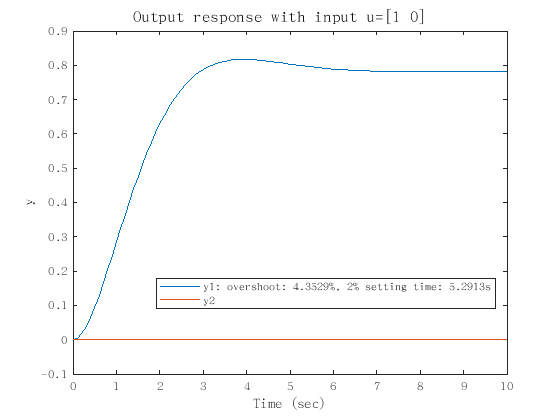
\includegraphics[width=8cm]{fig30.png}
		\end{minipage}
		\begin{minipage}[t]{0.48\textwidth}
			\centering
			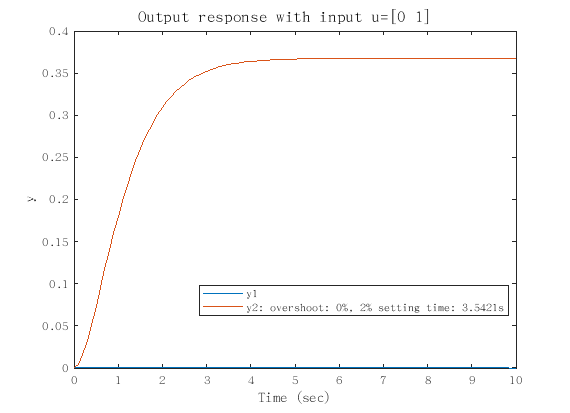
\includegraphics[width=8cm]{fig31.png}
		\end{minipage}
		\caption{Step response for the decoupled system (zero initial condition)}
		\label{fig21}
	\end{figure}

	Fig.~\ref{fig22} also gives the system response with non-zero initial state $x_{0}$. The closed-loop system is external(BIBO) stable. 
	
	\begin{figure}[H]
		\centering
		\begin{minipage}[t]{0.48\textwidth}
			\centering
			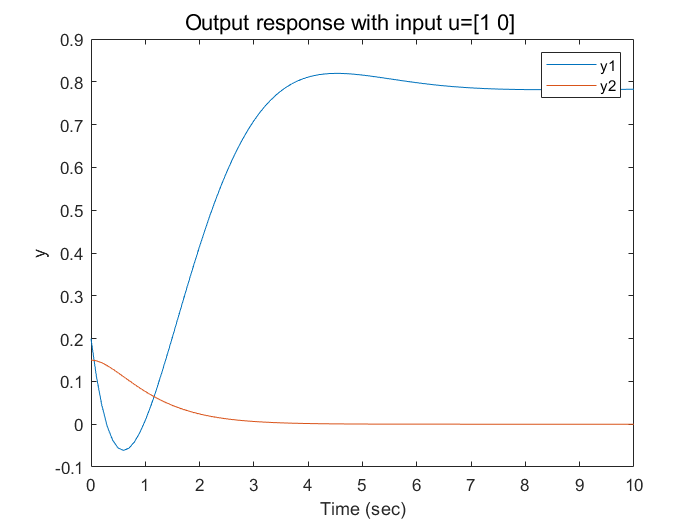
\includegraphics[width=6cm]{fig32.png}
		\end{minipage}
		\begin{minipage}[t]{0.48\textwidth}
			\centering
			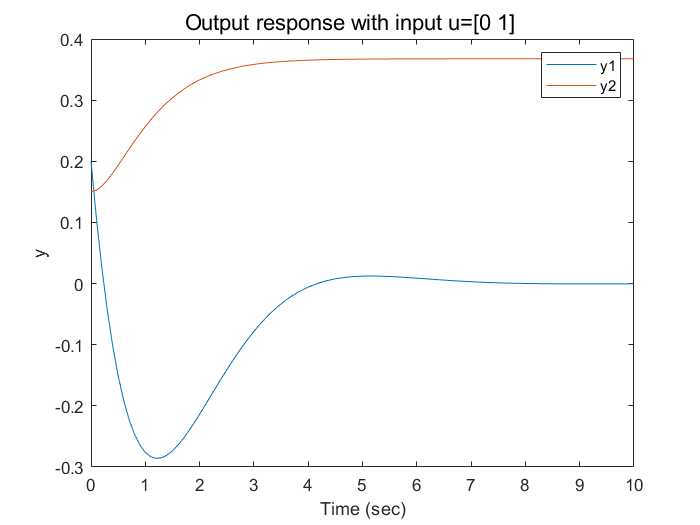
\includegraphics[width=6cm]{fig33.png}
		\end{minipage}
		\begin{minipage}[t]{0.48\textwidth}
			\centering
			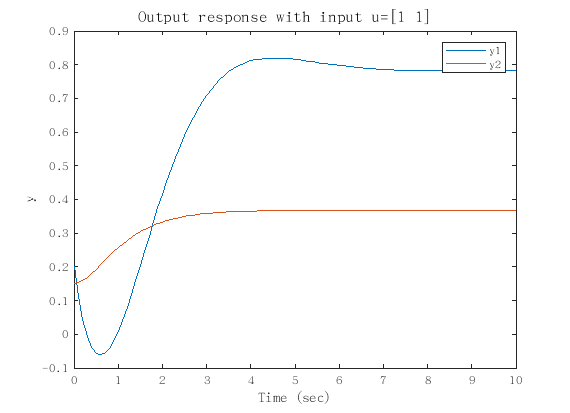
\includegraphics[width=6cm]{fig34.png}
		\end{minipage}
		\begin{minipage}[t]{0.48\textwidth}
			\centering
			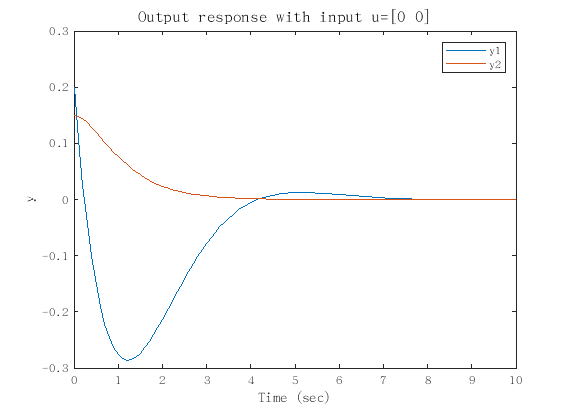
\includegraphics[width=6cm]{fig35.png}
		\end{minipage}
		\caption{Step response of the decoupled system for 4 combination cases of inputs (non-zero initial condition)}
		\label{fig22}
	\end{figure}
	
	However, the state feedback controller can't ensure the internal stability. To investigate it, we utilize the state observer to check the six state responses after given a step signal in the first channel. The response curve is given in Fig~\ref{fig23}, where the second and fifth states are unstable by the decoupling controller and the system is only BIBO stable but not internally stable. The poles of the system is also checked and one has positive real part (2.4821), which results in the instability.
	
	 \begin{figure}[H]
	 	\centering
	 	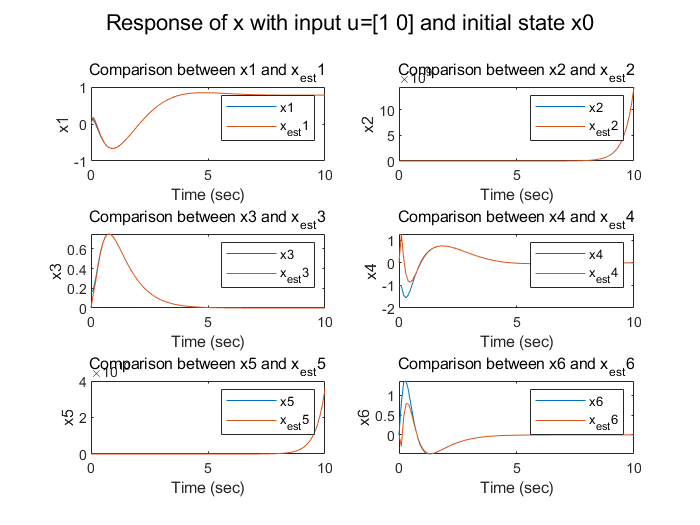
\includegraphics[width=8cm]{fig36.png}
	 	\caption{Six state response of the decoupled system (step signal in the first channel)}
	 	\label{fig23}
	 \end{figure}
	
	
	
	
	\section{Conclusion}
	\section*{Acknowledgments}
	%MS++++++++++++++++++++++++++++++ Reference ++++++++++++++++++
	%% 参考文献请看下一节详细介绍。
	
	\bibliographystyle{IEEEtran}
	
	\bibliography{ref_5401}{}
	
\end{document}